\documentclass[10pt,aspectratio=169]{beamer}

\usetheme{default}
\usecolortheme{default}
\setbeamertemplate{navigation symbols}{}
\usepackage{appendixnumberbeamer}
\setbeamertemplate{footline}[frame number]
\usepackage{booktabs}
\usepackage{graphicx}
\usepackage{array}
\usepackage{amsmath}
\usepackage{tikz}
\usepackage[dvipsnames]{xcolor}
\graphicspath{{../project/output/figures/}}

\definecolor{darkgreen}{RGB}{0,66,37}
\definecolor{forestlight}{RGB}{239,246,242}
\definecolor{forestgray}{RGB}{82,91,87}
\definecolor{fireaccent}{RGB}{174,68,36}
\definecolor{citationblue}{RGB}{0,102,204}
\newcommand{\citelink}[2]{\textcolor{citationblue}{\hyperlink{#2}{#1}}}
\newcommand{\prefcell}[1]{\alt<2->{\begingroup\setlength{\fboxsep}{1pt}\setlength{\fboxrule}{0.7pt}\textcolor{fireaccent}{\fbox{\textcolor{black}{\strut #1}}}\endgroup}{#1}}

\hypersetup{
  colorlinks=true,
  linkcolor=darkgreen,
  urlcolor=darkgreen
}
\pdfstringdefDisableCommands{%
  \def\translate#1{#1}%
}

\setbeamercolor{normal text}{fg=black,bg=white}
\setbeamercolor{title}{fg=darkgreen}
\setbeamercolor{subtitle}{fg=forestgray}
\setbeamercolor{frametitle}{fg=darkgreen,bg=white}
\setbeamercolor{framesubtitle}{fg=forestgray}
\setbeamercolor{structure}{fg=darkgreen}
\setbeamercolor{item}{fg=darkgreen}
\setbeamercolor{alerted text}{fg=fireaccent}
\setbeamercolor{block title}{fg=white,bg=darkgreen}
\setbeamercolor{block body}{fg=black,bg=forestlight}
\setbeamerfont{title}{size=\large,series=\bfseries}
\setbeamerfont{frametitle}{size=\large,series=\bfseries}
\setbeamerfont{framesubtitle}{size=\normalsize}
\setbeamerfont{normal text}{size=\small}
\setbeamertemplate{caption}[numbered]
\setbeamertemplate{footline}{
  \hfill\insertframenumber\,/\,\inserttotalframenumber
  \hspace{0.5em}
  \vspace{0.5em}
}
\newsavebox{\fuelfigbox}

\title{Do Fuel Reduction Treatments Prevent Wildfire Disasters in the U.S. Wildland--Urban Interface?}
\subtitle{}
\author{\texorpdfstring{Yanxu Long\textsuperscript{1} \and Stephen Polasky\textsuperscript{1} \and Dalia Abbas Iossifov\textsuperscript{2}}{Yanxu Long, Stephen Polasky, Dalia Abbas Iossifov}}
\date{}

\begin{document}

\begin{frame}[plain]
  \setbeamertemplate{headline}{}
  \setbeamertemplate{footline}{}
  \centering
  \vspace{1.3cm}
  {\Large \textcolor{darkgreen}{\textbf{Do Fuel Reduction Treatments Prevent Wildfire Disasters in the U.S. Wildland--Urban Interface?}}} \\[0.9em]
  \vspace{1.6em}
  {\normalsize Yanxu Long\textsuperscript{1} \quad Stephen Polasky\textsuperscript{1} \quad Dalia Abbas Iossifov\textsuperscript{2}} \\[0.7em]
  {\scriptsize \textsuperscript{1} University of Minnesota} \\[0.2em]
  {\scriptsize \textsuperscript{2} USDA Forest Service}
  \vfill
  {\small 2026 AAEA Annual Meeting} \\[0.25em]
  {\small Kansas City, MO}
\end{frame}

% NatCap Lab: introductory research slides (2026-11-02)
\begin{frame}{My Research: Natural Capital}
  \begin{columns}[c,onlytextwidth]
    \begin{column}{0.47\textwidth}
      \centering
      % Image is stored outside the Git repository in the project output directory.
      \IfFileExists{/Users/long/Files/my_devstack/fuel_reduction_wildfire/project/output/slides/slides_figures/SDSS.png}{%
        \includegraphics[
          width=\linewidth,
          height=0.77\textheight,
          keepaspectratio
        ]{/Users/long/Files/my_devstack/fuel_reduction_wildfire/project/output/slides/slides_figures/SDSS.png}%
      }{%
        \fbox{\parbox[c][0.52\textheight][c]{0.91\linewidth}{%
          \centering\small Figure not found:\\[0.3em] SDSS.png%
        }}%
      }
    \end{column}
    \begin{column}{0.49\textwidth}
      \raggedright
      {\small \href{https://www.econ.cam.ac.uk/people/academic/partha-dasgupta}{\textcolor{black}{\textbf{Professor Sir Partha Dasgupta}}}}\par
      \vspace{1.0em}
      {\Large\bfseries\color{black} On Natural Capital:}\par
      \vspace{0.6em}
      {\large\bfseries\color{black} The Value of the World Around Us}\par
      \vspace{0.6em}
      {\normalsize\bfseries\color{black} Transforming Economics to Value Nature and Combat Climate Change}\par
    \end{column}
  \end{columns}
\end{frame}

\begin{frame}{My Research: Wildfire Risk and Natural Capital}
  \raggedright
  \begin{block}{Research focus}
    How can land-management decisions protect communities and the natural capital on which they depend?
  \end{block}
  \vspace{0.5em}
  \begin{itemize}
    \setlength{\itemsep}{1.0em}
    \item \textbf{Natural capital:} Forest landscapes provide ecosystem services while also facing disturbance risks.
    \item \textbf{Management:} Fuel reduction treatments may alter wildfire behavior and pathways.
    \item \textbf{Policy evaluation:} Assess whether treatments reduce wildfire exposure and damage in wildland--urban interface communities.
  \end{itemize}
\end{frame}

\begin{frame}{Introduction}
  \raggedright
  \begin{itemize}
    \item Wildfires cause huge damages in the US. In 2000--2024, each year about \textbf{69,384} wildfires, about \textbf{7 million} acres burned, around \textbf{6,620} structures destroyed, and \textbf{41,380} wildfire-smoke excess deaths (\citelink{National Interagency Fire Center, 2026}{ref:nifc2025}; \citelink{Chen et al., 2024}{ref:chen2024}; \citelink{Qiu et al., 2025}{ref:qiu2025}).
    \item Damages intensify under a warming climate and changing fire regimes (\citelink{Westerling et al., 2006}{ref:westerling2006}; \citelink{Abatzoglou \& Williams, 2016}{ref:abatzoglou2016}).
    \item Wildland--urban interface (WUI) communities face high exposure where wildland fuels meet homes and fires spread into built environments (\citelink{Radeloff et al., 2018}{ref:radeloff2018}; \citelink{Chen et al., 2024}{ref:chen2024}; \citelink{Balch et al., 2024}{ref:balch2024}).
  \end{itemize}

  \vspace{0.45em}
\begin{columns}[T,onlytextwidth]
    \begin{column}{0.48\textwidth}
      \centering
      \includegraphics[width=\linewidth,height=0.4\textheight]{MN_camphousefire_fixed.png}
    \end{column}
    \begin{column}{0.48\textwidth}
      \centering
      \includegraphics[width=\linewidth,height=0.4\textheight]{ca_wildfire_converted.png}
    \end{column}
  \end{columns}
\end{frame}

\begin{frame}{Fire Behavior}
  {Fire regime = Ignition + fuels + topography + climate/weather}
  \centering
  \vspace{0.10cm}
  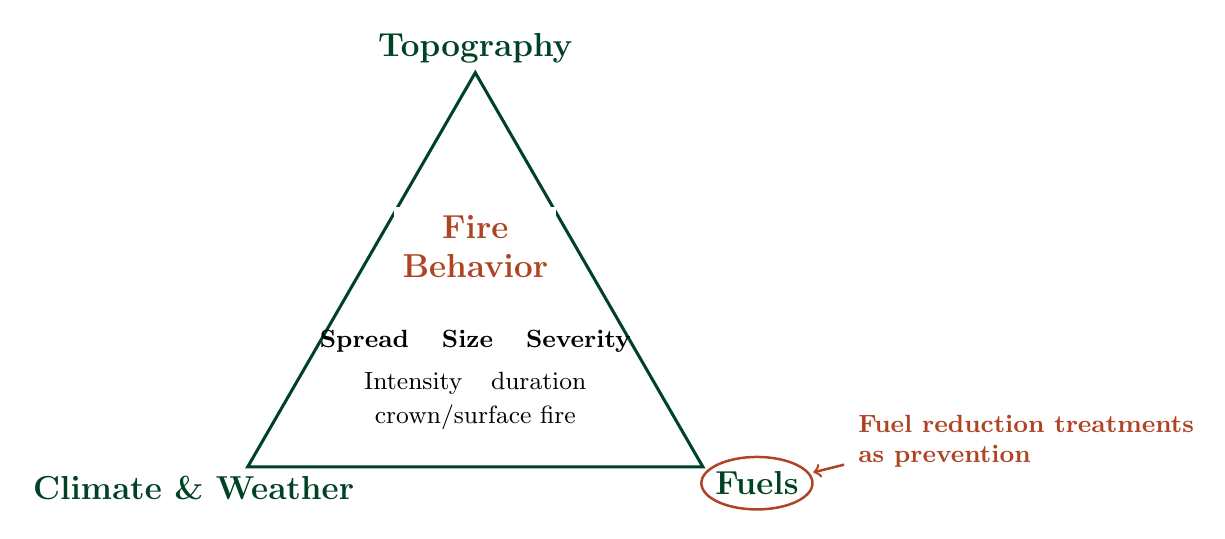
\begin{tikzpicture}[x=0.98cm,y=0.98cm, every node/.style={font=\small}]
    \coordinate (topography) at (0,3.20);
    \coordinate (climate) at (-2.95,-1.91);
    \coordinate (fuels) at (2.95,-1.91);
    \draw[line width=1.1pt, darkgreen] (topography) -- (climate) -- (fuels) -- cycle;

    \node[align=center, text=darkgreen, font=\bfseries\large, fill=white, inner sep=2pt] at (0,3.52) {Topography};
    \node[align=center, text=darkgreen, font=\bfseries\large, fill=white, inner sep=2pt] at (-3.65,-2.18) {Climate \& Weather};
    \node[align=center, text=darkgreen, font=\bfseries\large, fill=white, inner sep=2pt] at (3.65,-2.12) {Fuels};
    \visible<2->{
      \draw[line width=0.9pt, fireaccent] (3.65,-2.12) ellipse [x radius=0.72, y radius=0.34];
      \node[anchor=west, align=left, text=fireaccent, font=\bfseries\small, fill=white, inner sep=1pt] (fuelreduction) at (4.92,-1.58) {Fuel reduction treatments\\as prevention};
      \draw[->, line width=0.9pt, fireaccent] (4.78,-1.88) -- (4.38,-1.98);
    }

    \node[align=center, text=fireaccent, font=\bfseries\large, fill=white, inner sep=3pt] at (0,0.95) {Fire\\Behavior};
    \node[align=center, text=black, font=\bfseries\small, inner sep=3pt] at (0,-0.28)
      {Spread \hspace{0.45em} Size \hspace{0.45em} Severity};
    \node[align=center, text=black, font=\normalfont\small, fill=white, inner sep=3pt] at (0,-0.82)
      {Intensity \hspace{0.45em} duration};
    \node[align=center, text=black, font=\normalfont\small, fill=white, inner sep=3pt] at (0,-1.26)
      {crown/surface fire};
  \end{tikzpicture} \\
\textit{Notes:} This figure is revised from \citelink{Miller et al., 2013}{ref:miller2013}.
\end{frame}

\begin{frame}{Fuel Reduction Treatments}
\begin{columns}[T,onlytextwidth]
  \begin{column}{0.35\textwidth}
    \begin{itemize}
    \item Fuel reduction \textbf{lowers fuels} through prescribed fire and mechanical treatment such as thinning and pruning (\citelink{Agee \& Skinner, 2005}{ref:agee2005}; \citelink{U.S. Forest Service, 2022}{ref:usfs2022}).
    \item Lowered fuels \textbf{reduce} ignition-to-crown transition, spread, intensity, and severity in treated areas (\citelink{Agee \& Skinner, 2005}{ref:agee2005}; \citelink{Stephens et al., 2012}{ref:stephens2012}; \citelink{Plantinga et al., 2022}{ref:plantinga2022}; \citelink{Strabo et al., 2026}{ref:strabo2026}).
    \end{itemize}
  \end{column}
  \begin{column}{0.65\textwidth}
    \centering
    \sbox{\fuelfigbox}{\includegraphics[width=\linewidth,height=0.7\textheight,keepaspectratio]{fuel_reductiment.png}}
    \usebox{\fuelfigbox}
    \vspace{0.1cm}
    \parbox{\wd\fuelfigbox}{\scriptsize \textit{Notes:} Fig. 6.4. 2011 Wallow Fire near Alpine, Arizona. Photo by U.S. Forest Service. Source: Chapter 6, Regional Highlights of Climate Change.}
  \end{column}
\end{columns}
\end{frame}

\begin{frame}{Research Questions}
  \begin{columns}[T,onlytextwidth]
    \begin{column}{0.5\textwidth}
      \begin{itemize}
        \item When wildfires spread, do fuel reduction treatments interrupt the fire path to WUI communities?
        \begin{itemize}
          \item Prevent WUI burning?
          \item Reduce burned area?
          \item Lower burn severity?
        \end{itemize}
        \item If so, what treatment types work best and which types of communities are protected most effectively?
      \end{itemize}
    \end{column}
    \begin{column}{0.425\textwidth}
      \centering
      \textbf{Like a Blockus game}
      \vspace{-0.25em}
      \par\includegraphics[width=\linewidth,height=0.68\textheight,keepaspectratio]{Blokus.png}
    \end{column}
  \end{columns}
\end{frame}

\begin{frame}{Preview of Main Findings}
  \begin{itemize}
    \item Fuel treatment prevents wildfire disasters in the WUI.
      \begin{itemize}
        \item Reduces burning probability by 4.3\%.
        \item Reduces burned area by about 22.3\%.
        \item Lowers burn severity by 0.14 index points.
      \end{itemize}
    \item Both prescribed fire and mechanical treatment show consistent negative estimates.
      \begin{itemize}
        \item Prescribed fire reduces burning probability more than mechanical treatment.
        \item Mechanical treatment is more effective for burned acres and burn severity.
      \end{itemize}
    \item Fuel treatments have stronger effects for interface WUI than intermix WUI.
    \item Treatment effects persist over time.
    \item When treatment covers less than 100\% of the fire path, effects are uncertain.
  \end{itemize}
\end{frame}

\begin{frame}{Data}
  \begin{itemize}
    \item Setting: US National Forest fires and nearby WUI polygons, 2000--2024.
    \item Treatments: completed Forest Service Activity Tracking System (FACTS) hazardous-fuel polygons before fire exposure.
    \item Outcomes: any burn, log burned acres, and burn severity from Monitoring Trends in Burn Severity (MTBS) in WUI communities (\citelink{Radeloff et al., 2018}{ref:radeloff2018}).
    \item Controls: ignition-date wind; Parameter-elevation Regressions on Independent Slopes Model (PRISM) weather; USFS roads and primary highways; LANDFIRE fuels/terrain; path elevation; and prior FACTS wildfire-path exposure.
  \end{itemize}
\end{frame}

\begin{frame}{Data}
  \centering
  {\scriptsize \textit{Figure:} WUI-proximate wildfires with fuel treatment.}

  \vspace{0.15em}
  \includegraphics[width=0.95\textwidth,height=0.78\textheight,keepaspectratio]{map_mtbs_fires_wui_2p41402km_main_regression_distribution_final.png}
\end{frame}

\begin{frame}{Summary Statistics}
  \centering
  {\small Table 1---Baseline summary statistics}

  \vspace{0.15em}
  \scriptsize
  \setlength{\tabcolsep}{2.5pt}
  \renewcommand{\arraystretch}{0.86}
  \resizebox{0.98\textwidth}{!}{%
  \begin{tabular}{@{}>{\raggedright\arraybackslash}p{0.43\textwidth}rrrr@{}}
  \specialrule{0.03em}{0pt}{0.08em}
  \specialrule{0.03em}{0pt}{0.35em}
  Variable & Treatment Mean & Treatment SD & Control Mean & Control SD \\
  \midrule
  \multicolumn{5}{@{}l}{\textit{Panel A. Main outcomes}} \\
  Any burn (\%) & 18.52 & 38.86 & 18.35 & 38.71 \\
  Log(1 + burned acres) & 0.31 & 0.89 & 0.48 & 1.28 \\
  Burned acres & 2.87 & 15.89 & 13.89 & 115.46 \\
  Burn severity index & 0.26 & 0.71 & 0.36 & 0.88 \\
  \\[-0.3em]
  \multicolumn{5}{@{}l}{\textit{Panel B. Treatment rule}} \\
  100\% coverage treatment & 1.00 & 0.00 & 0.00 & 0.00 \\
  Angular coverage (\%) & 100.00 & 0.00 & 0.00 & 0.00 \\
  Treatment acres & 971.11 & 6292.96 & 0.00 & 0.00 \\
  \\[-0.3em]
  \multicolumn{5}{@{}l}{\textit{Panel C. WUI exposure and geometry}} \\
  Distance to ignition (km) & 5.42 & 5.44 & 10.65 & 8.10 \\
  WUI area (acres) & 39.36 & 165.56 & 70.74 & 255.79 \\
  Intermix WUI (\%) & 42.07 & 49.39 & 35.26 & 47.78 \\
  \\[-0.3em]
  \multicolumn{5}{@{}l}{\textit{Panel D. Terrain and path controls}} \\
  Nearest-point slope (degrees) & 6.44 & 6.59 & 5.11 & 5.75 \\
  Net elevation change (m) & -229.53 & 460.87 & -278.97 & 384.34 \\
  \midrule
  Observations & \multicolumn{2}{c}{1,091} & \multicolumn{2}{c}{28,150} \\
  Severity observations & \multicolumn{2}{c}{902} & \multicolumn{2}{c}{21,748} \\
  \bottomrule
  \end{tabular}}

  \vspace{0.15em}
  \begin{minipage}{0.98\textwidth}
    \tiny
    \textit{Notes:} Values use the same restricted sample as Table 2. Treatment is exact-100 percent WUI-facing angular-block coverage within 1.5 miles of WUI, completed prior 1--5 years before the fire. Controls have zero WUI-facing path coverage. Severity rows use valid MTBS severity observations.
  \end{minipage}
  \renewcommand{\arraystretch}{1}
\end{frame}

\begin{frame}{Empirical Strategy}
\framesubtitle{Spatial DID estimation}
  \begin{columns}[T]
    \begin{column}{0.5\textwidth}
      \begin{itemize}
        \item Following \citelink{Strabo et al. (2026)}{ref:strabo2026}, we adopt a spatial difference-in-differences strategy by defining 0.5 km distance bins along the path from fire ignition points to WUI polygons.
        \item Distance bins can be treated as time in canonical DID.
        \item Compare treated and control WUI polygons within the same fire-by-direction cell and distance bin.
      \end{itemize}
    \end{column}
    \begin{column}{0.5\textwidth}
      \begin{figure}
        \centering
        \includegraphics[width=\linewidth,height=0.63\textheight,keepaspectratio]{/Users/long/Files/my_devstack/fuel_reduction_wildfire/project/output/figures/tree_ring_diagram.png}
      \end{figure}
      {\tiny Source: Science Education Resource Center, Carleton College}
    \end{column}
  \end{columns}
\end{frame}

\begin{frame}{Empirical Strategy}
\textbf{Treatment:} completed fuel-reduction work before the fire up to 1.5 miles on the WUI-facing ignition-to-WUI path, within the fire-perimeter threat buffer (Baseline: 1.5 miles \(\approx\) 2.4 km). \\
   \vspace{-0.5em}
   \begin{figure}
    \centering
    \includegraphics[width=1\textwidth,height=0.8\textheight,keepaspectratio]{/Users/long/Files/my_devstack/fuel_reduction_wildfire/project/output/figures/nearestpoint_mechanism_conceptual_diagram_outcome_cases.png}
  \end{figure}
  \vspace{0em}
\end{frame}

\begin{frame}{Empirical Strategy}
  \begin{columns}[T,onlytextwidth]
    \begin{column}{0.25\textwidth}
      \textbf{Comparison at:}
      \begin{enumerate}
        \item Same fire
        \item Same fire direction
        \item Same distance bin
      \end{enumerate}
    \end{column}
    \begin{column}{0.75\textwidth}
      \vspace{-3em}
      \begin{figure}
        \centering
        \includegraphics[width=\linewidth,height=1\textheight,keepaspectratio]{/Users/long/Files/my_devstack/fuel_reduction_wildfire/project/output/figures/nearestpoint_mechanism_4_direction_distance_bins.png}
      \end{figure}
    \end{column}
  \end{columns}
\end{frame}

\begin{frame}{Empirical Strategy}
  \[
  Y_{fw}=\beta D_{fw} + \alpha_f+\gamma_d+\mathrm{dist}_{b(f,w)}+\mathbf{X}'_{fw}\mathbf{\theta}+\varepsilon_{fw}.
  \]
  \begin{itemize}
    \item $D_{fw}=1$ for prior-fire treatment in the WUI-facing ignition-to-WUI path.
    \item $\beta$ is the average treatment effect on WUI burning outcomes.
    \item $\alpha_f$ are fire fixed effects.
    \item $\gamma_d$ are fire-direction fixed effects.
    \item $\mathrm{dist}_{b(f,w)}$ are distance-bin fixed effects.
    \item $f$ indexes fires, $d$ indexes directions, and $w$ indexes WUI polygons.
    \item $\mathbf{X}_{fw}$ are controls for weather, fuels, terrain, roads, path elevation, and prior wildfire-path exposure.
    \item Estimation uses the Borusyak--Jaravel--Spiess (BJS) imputation estimator (\citelink{Borusyak et al., 2024}{ref:borusyak2024}).
    \item Standard errors are clustered by fire.
  \end{itemize}
\end{frame}

\begin{frame}{Baseline Results}
  \centering
  {\small Table 2---Baseline results}

  \vspace{0.1em}
  \small
  \setlength{\tabcolsep}{2.2pt}
  \renewcommand{\arraystretch}{1.0}
  \resizebox{\textwidth}{!}{%
  \begin{tabular}{@{}>{\raggedright\arraybackslash}p{0.13\textwidth}*{9}{>{\centering\arraybackslash}p{0.093\textwidth}}@{}}
  \specialrule{0.03em}{0pt}{0.08em}
  \specialrule{0.03em}{0pt}{0.35em}
  Dependent & \multicolumn{3}{c}{Any burn} & \multicolumn{3}{c}{Log} & \multicolumn{3}{c}{Burn severity} \\
  variable & \multicolumn{3}{c}{(\%)} & \multicolumn{3}{c}{(1 + burned acres)} & \multicolumn{3}{c}{index} \\
  \cmidrule(lr){2-4}
  \cmidrule(lr){5-7}
  \cmidrule(lr){8-10}
   & (1) & (2) & (3) & (4) & (5) & (6) & (7) & (8) & (9) \\
  \midrule
Treatment & -5.85** & -4.44* & \prefcell{-4.33*} & -0.25*** & -0.26*** & \prefcell{-0.25***} & -0.14*** & -0.14*** & \prefcell{-0.14***} \\
 & (2.29) & (2.62) & (2.63) & (0.08) & (0.07) & (0.07) & (0.04) & (0.05) & (0.05) \\
  Fire FE & $\checkmark$ & $\checkmark$ & $\checkmark$ & $\checkmark$ & $\checkmark$ & $\checkmark$ & $\checkmark$ & $\checkmark$ & $\checkmark$ \\
  \mbox{Dist.-bin FE} & $\checkmark$ & $\checkmark$ & $\checkmark$ & $\checkmark$ & $\checkmark$ & $\checkmark$ & $\checkmark$ & $\checkmark$ & $\checkmark$ \\
  \mbox{Fire Direction FE} &  & $\checkmark$ & $\checkmark$ &  & $\checkmark$ & $\checkmark$ &  & $\checkmark$ & $\checkmark$ \\
  Controls &  &  & $\checkmark$ &  &  & $\checkmark$ &  &  & $\checkmark$ \\
  \midrule
  \mbox{Mean dep. var.} & \multicolumn{3}{c}{18.36} & \multicolumn{3}{c}{0.47} & \multicolumn{3}{c}{0.36} \\
  Fires & \multicolumn{3}{c}{474} & \multicolumn{3}{c}{474} & \multicolumn{3}{c}{302} \\
  \mbox{Treated Obs.} & \multicolumn{3}{c}{1,091} & \multicolumn{3}{c}{1,091} & \multicolumn{3}{c}{902} \\
  \mbox{Control Obs.} & \multicolumn{3}{c}{28,150} & \multicolumn{3}{c}{28,150} & \multicolumn{3}{c}{21,748} \\
  \bottomrule
  \end{tabular}}
  \vspace{0.15em}

  \begin{minipage}{0.985\textwidth}
    \tiny
  \textit{Notes:} Sample uses the exact 2.41402 km fire-perimeter threat buffer. Treatment equals 100 percent WUI-facing angular-block coverage within 1.5 miles of WUI, completed prior 1--5 years before the fire. Controls have zero WUI-facing path coverage; incomplete or farther positive coverage is omitted. Within each outcome, columns add fire and distance-bin FE, fire-direction FE, then controls. Standard errors are clustered by fire. Stars mark p-values: *** p $<$ 0.01; ** p $<$ 0.05; * p $<$ 0.10. Any burn is in percentage points; log burned acres is in log units; burn severity is in index points. Means are unconditional. Severity outcomes use rows with valid MTBS severity values.
  \end{minipage}
\vspace{0.2em}
  \begin{center}
    \hyperlink{appendix-event-study}{\beamerbutton{Event Study: Any burn}}
    \hyperlink{appendix-event-study-acres}{\beamerbutton{Event Study: Burned acres}}
    \hyperlink{appendix-event-study-severity}{\beamerbutton{Event Study: Severity}}
  \end{center}
  \renewcommand{\arraystretch}{1}
\end{frame}

\begin{frame}{Fuel Reduction Treatment Types}
  \begin{columns}[T,onlytextwidth]
    \begin{column}{0.48\textwidth}
      \centering
      \includegraphics[width=\linewidth,height=0.52\textheight,keepaspectratio]{slides/fuel_treatment_prescribed_fire.jpg}

      \vspace{0.08cm}
      \textbf{Prescribed fire}

      \scriptsize Burns leaf litter, grasses, shrubs, and other surface fuels under controlled conditions.\\
      \tiny Source: National Park Service (2024).
    \end{column}
    \begin{column}{0.48\textwidth}
      \centering
      \includegraphics[width=\linewidth,height=0.52\textheight,keepaspectratio]{slides/fuel_treatment_cut_pile.jpg}

      \vspace{0.08cm}
      \textbf{Mechanical thinning}

      \scriptsize Cuts small trees and ladder fuels that connect surface fire to canopy.\\
      \tiny Source: Rocky Mountain National Park, via Sky-Hi News (2024).
    \end{column}
  \end{columns}
\end{frame}




\begin{frame}{Fuel Reduction Treatment-Type Heterogeneity Results}
  
    \begin{itemize}
    \item Prescribed fire shows stronger protection against any WUI burning.
    \item Mechanical treatment shows larger effects for burned acres and burn severity.
  \end{itemize}
  \centering
  {\small Table 3---Treatment-type heterogeneity results}


  \small
  \setlength{\tabcolsep}{2.8pt}
  \renewcommand{\arraystretch}{1.0}
  \resizebox{\textwidth}{!}{%
  \begin{tabular}{@{}>{\raggedright\arraybackslash}p{0.16\textwidth}*{6}{>{\centering\arraybackslash}p{0.12\textwidth}}@{}}
  \specialrule{0.03em}{0pt}{0.08em}
  \specialrule{0.03em}{0pt}{0.35em}
  Dependent & \multicolumn{2}{c}{Any burn} & \multicolumn{2}{c}{Log} & \multicolumn{2}{c}{Burn severity} \\
  variable & \multicolumn{2}{c}{(\%)} & \multicolumn{2}{c}{(1 + burned acres)} & \multicolumn{2}{c}{index} \\
  \cmidrule(lr){2-3}
  \cmidrule(lr){4-5}
  \cmidrule(lr){6-7}
  Type & Prescribed & Mechanical & Prescribed & Mechanical & Prescribed & Mechanical \\
  \midrule
  Treatment & -5.74*** & -3.73 & -0.11*** & -0.32*** & -0.10*** & -0.16** \\
   & (1.56) & (3.40) & (0.04) & (0.10) & (0.03) & (0.07) \\
  \midrule
  \mbox{Mean dep. var.} & 18.27 & 18.44 & 0.48 & 0.48 & 0.36 & 0.36 \\
  Fires & 463 & 464 & 463 & 464 & 301 & 302 \\
  \mbox{Treated Obs.} & 392 & 702 & 392 & 702 & 321 & 584 \\
  \mbox{Control Obs.} & 28,150 & 28,150 & 28,150 & 28,150 & 21,748 & 21,748 \\
  \bottomrule
  \end{tabular}}
  \vspace{0.15em}

  \begin{minipage}{1\textwidth}
    \tiny
  \textit{Notes:} Treatment type is based on the first exact-100 percent WUI-facing angular-block treatment within 1.5 miles of WUI, completed prior 1--5 years before the fire. Controls have zero WUI-facing angular coverage. Each column reports the preferred specification with fire FE, distance-bin FE, four fire-direction FE, and controls. Standard errors are clustered by fire. Stars mark p-values: *** p $<$ 0.01; ** p $<$ 0.05; * p $<$ 0.10.
  \end{minipage}
  \renewcommand{\arraystretch}{1}
\end{frame}


\begin{frame}{Fuel Reduction Treatment-Type Mechanism}
  \begin{columns}[T,onlytextwidth]
    \begin{column}{0.62\textwidth}
      \centering
      \begin{tikzpicture}
        \node[inner sep=0pt] (photo) {\includegraphics[width=\linewidth,height=0.68\textheight,keepaspectratio]{sycu_photos_2024_10_treatments_photo.png}};
        \node[anchor=north west, align=left, fill=white, fill opacity=0.82, text opacity=1, rounded corners=1pt, inner sep=3pt, font=\bfseries\tiny, text=darkgreen] at ([xshift=0.25cm,yshift=-0.25cm]photo.north west) {Mechanical Treatment\\+ Prescribed Fire};
        \node[anchor=north east, align=right, fill=white, fill opacity=0.82, text opacity=1, rounded corners=1pt, inner sep=3pt, font=\bfseries\tiny, text=fireaccent] at ([xshift=-0.25cm,yshift=-0.25cm]photo.north east) {Mechanical\\Treatment only};
      \end{tikzpicture}
      \vspace{0.1em}
      \begin{minipage}{\linewidth}
        \tiny
        \textit{Notes:} Location: Bootleg Fire, Fremont--Winema National Forest, Oregon, taken in 2021. Photo credit: John F. Marshall LLC. Source: Science You Can Use in 5 Minutes, USDA Forest Service Rocky Mountain Research Station (October 2024).
      \end{minipage}
    \end{column}
    \begin{column}{0.36\textwidth}
      \scriptsize
      \textbf{Mechanism}
      \vspace{0.2em}
      \begin{itemize}
        \item \textbf{Crown fire:} typically more intense and damaging than surface fire because it burns canopy fuels and can spread faster (\citelink{Scott \& Reinhardt, 2001}{ref:scott2001}; \citelink{Graham et al., 2004}{ref:graham2004}).
        \item \textbf{Mechanical thinning:} removes ladder fuels and reduces surface-to-crown transition.
        \item \textbf{Surface fire:} can still spread if fine surface fuels remain.
      \end{itemize}

      \vspace{0.8em}
      \textbf{Policy implication:} Mechanical treatment and prescribed fire should be implemented together.
    \end{column}
  \end{columns}
\end{frame}



\begin{frame}{Treatment-Year Heterogeneity Results}
  
  Treatments completed 2.5--5 years before the fire still reduce burned acres and burn severity, although the effect on burn probability is not statistically significant.

  \vspace{0.2em}
  {\centering\small Table 4---Treatment-year heterogeneity results\par}

  \vspace{0.25em}
  \small
  \setlength{\tabcolsep}{5pt}
  \renewcommand{\arraystretch}{1.12}
  \resizebox{0.92\textwidth}{!}{%
  \begin{tabular}{@{}>{\raggedright\arraybackslash}p{0.16\textwidth}*{6}{>{\centering\arraybackslash}p{0.12\textwidth}}@{}}
  \specialrule{0.03em}{0pt}{0.08em}
  \specialrule{0.03em}{0pt}{0.35em}
  Dependent & \multicolumn{2}{c}{Any burn} & \multicolumn{2}{c}{Log} & \multicolumn{2}{c}{Burn severity} \\
  variable & \multicolumn{2}{c}{(\%)} & \multicolumn{2}{c}{(1 + burned acres)} & \multicolumn{2}{c}{index} \\
  \cmidrule(lr){2-3}
  \cmidrule(lr){4-5}
  \cmidrule(lr){6-7}
  Window & \shortstack{$t-2.5$\\to $t0$} & \shortstack{$t-5$\\to $t-2.5$} & \shortstack{$t-2.5$\\to $t0$} & \shortstack{$t-5$\\to $t-2.5$} & \shortstack{$t-2.5$\\to $t0$} & \shortstack{$t-5$\\to $t-2.5$} \\
  \midrule
  Treatment & -2.58** & -5.80 & -0.148*** & -0.341*** & -0.101*** & -0.170** \\
   & (1.27) & (4.53) & (0.047) & (0.121) & (0.035) & (0.078) \\
  \midrule
  \mbox{Mean dep. var.} & 18.36 & 18.36 & 0.47 & 0.47 & 0.36 & 0.36 \\
  Fires & 474 & 474 & 474 & 474 & 302 & 302 \\
  \mbox{Treated Obs.} & 443 & 648 & 443 & 648 & 382 & 520 \\
  \mbox{Control Obs.} & 28,150 & 28,150 & 28,150 & 28,150 & 21,748 & 21,748 \\
  \bottomrule
  \end{tabular}}

  \vspace{0.35em}
  \begin{minipage}{0.86\textwidth}
    \tiny
    \textit{Notes:} Preferred specification includes fire FE, distance-bin FE, four fire-direction FE, and controls. Treatment is exact-100 percent WUI-facing angular-block coverage within 1.5 miles of WUI, split at 2.5 years before the fire. Controls have zero WUI-facing path coverage. Standard errors are clustered by fire. Stars mark p-values: *** p $<$ 0.01; ** p $<$ 0.05; * p $<$ 0.10.
  \end{minipage}
  \renewcommand{\arraystretch}{1}
\end{frame}

\begin{frame}{WUI Types}
  \begin{columns}[T,onlytextwidth]
    \begin{column}{0.48\textwidth}
      \begin{block}{Intermix WUI}
        Housing and wildland vegetation occupy the same local landscape.
      \end{block}
      \vspace{0.4em}
      \begin{itemize}
        \item More vegetation within and around homes.
        \item Fire exposure can come from fuels embedded inside the community.
        \item Often higher baseline burn exposure.
      \end{itemize}
    \end{column}
    \begin{column}{0.48\textwidth}
      \begin{block}{Interface WUI}
        Housing lies next to a large wildland vegetation patch.
      \end{block}
      \vspace{0.4em}
      \begin{itemize}
        \item Built area is more clearly separated from wildland fuels.
        \item Fire exposure comes from the boundary between homes and vegetation.
        \item Treatment may matter through approach paths to that edge.
      \end{itemize}
    \end{column}
  \end{columns}

  \vspace{0.8em}
  {\scriptsize \textit{Definition:} Following the CONUS WUI classification (\citelink{Radeloff et al., 2018}{ref:radeloff2018}).}
\end{frame}

\begin{frame}{WUI-Type Heterogeneity Results}
  \centering
  {\small Table 5---WUI-type heterogeneity results}

  \vspace{0.1em}
  \small
  \setlength{\tabcolsep}{2.8pt}
  \renewcommand{\arraystretch}{1.0}
  \resizebox{\textwidth}{!}{%
  \begin{tabular}{@{}>{\raggedright\arraybackslash}p{0.16\textwidth}*{6}{>{\centering\arraybackslash}p{0.12\textwidth}}@{}}
  \specialrule{0.03em}{0pt}{0.08em}
  \specialrule{0.03em}{0pt}{0.35em}
  Dependent & \multicolumn{2}{c}{Any burn} & \multicolumn{2}{c}{Log} & \multicolumn{2}{c}{Burn severity} \\
  variable & \multicolumn{2}{c}{(\%)} & \multicolumn{2}{c}{(1 + burned acres)} & \multicolumn{2}{c}{index} \\
  \cmidrule(lr){2-3}
  \cmidrule(lr){4-5}
  \cmidrule(lr){6-7}
  WUI type & Intermix & Interface & Intermix & Interface & Intermix & Interface \\
  \midrule
  Treatment & -1.25 & -3.88* & -0.14 & -0.16*** & -0.09 & -0.09 \\
   & (2.45) & (2.26) & (0.08) & (0.05) & (0.06) & (0.06) \\
  \midrule
  \mbox{Mean dep. var.} & 32.40 & 10.62 & 1.01 & 0.18 & 0.66 & 0.20 \\
  Fires & 468 & 341 & 468 & 341 & 298 & 239 \\
  \mbox{Treated Obs.} & 459 & 632 & 459 & 632 & 331 & 571 \\
  \mbox{Control Obs.} & 9,926 & 18,224 & 9,926 & 18,224 & 7,540 & 14,208 \\
  \bottomrule
  \end{tabular}}
  \vspace{0.15em}

  \begin{minipage}{0.985\textwidth}
    \tiny
  \textit{Notes:} WUI type uses \texttt{wui\_is\_intermix}: intermix versus interface. Each column estimates the preferred specification within the WUI-type subsample, with fire FE, distance-bin FE, four fire-direction FE, and controls. Treatment is exact-100 percent WUI-facing angular-block coverage within 1.5 miles of WUI, completed prior 1--5 years before the fire. Controls have zero WUI-facing path coverage within the same WUI type. Standard errors are clustered by fire. Stars mark p-values: *** p $<$ 0.01; ** p $<$ 0.05; * p $<$ 0.10.
  \end{minipage}
  \renewcommand{\arraystretch}{1}
\end{frame}

\begin{frame}{Treatment Coverage}
  \centering
  \includegraphics[width=\textwidth,height=0.82\textheight,keepaspectratio]{nearestpoint_mechanism_4_direction_block_thresholds.png}
\end{frame}

\begin{frame}{Treatment Coverage Heterogeneity Results}
  \centering
  \begin{minipage}{1\textwidth}
    When treatment covers less than 100\% of the wildfire angular span, effects are uncertain.
  \end{minipage}

  \vspace{0.25em}
  {\small Table 6---Treatment coverage heterogeneity results}

  \vspace{0.1em}
  \small
  \setlength{\tabcolsep}{2.8pt}
  \renewcommand{\arraystretch}{1.05}
  \resizebox{\textwidth}{!}{%
  \begin{tabular}{@{}>{\raggedright\arraybackslash}p{0.20\textwidth}*{6}{>{\centering\arraybackslash}p{0.105\textwidth}}@{}}
  \specialrule{0.03em}{0pt}{0.08em}
  \specialrule{0.03em}{0pt}{0.35em}
  Dependent & \multicolumn{2}{c}{Any burn} & \multicolumn{2}{c}{Log} & \multicolumn{2}{c}{Burn severity} \\
  variable & \multicolumn{2}{c}{(\%)} & \multicolumn{2}{c}{(1 + burned acres)} & \multicolumn{2}{c}{index} \\
  \cmidrule(lr){2-3}
  \cmidrule(lr){4-5}
  \cmidrule(lr){6-7}
  Coverage & Estimate & SE & Estimate & SE & Estimate & SE \\
  \midrule
  Any positive $<100\%$ & -0.90 & (1.84) & 0.05 & (0.06) & -0.10 & (0.08) \\
  (0--25\%) & -0.16 & (1.84) & 0.19** & (0.07) & 0.07 & (0.12) \\
  \mbox{[25--50\%)} & 0.55 & (1.75) & 0.10 & (0.07) & -0.38*** & (0.15) \\
  \mbox{[50--75\%)} & -0.82 & (1.65) & -0.07 & (0.07) & 0.08 & (0.08) \\
  \mbox{[75--100\%)} & -3.19* & (1.90) & -0.08 & (0.06) & -0.14 & (0.10) \\
  \bottomrule
  \end{tabular}}
  \vspace{0.2em}

  \begin{minipage}{0.985\textwidth}
    \tiny
  \textit{Notes:} Preferred specification includes fire FE, distance-bin FE, four fire-direction FE, and controls. Treatment is WUI-facing angular-block coverage within 1.5 miles of WUI, completed prior 1--5 years before the fire. Exact 100 percent coverage is omitted from this bin check and used in the baseline table. Controls have zero WUI-facing path coverage. Standard errors are clustered by fire.
  \end{minipage}
  \renewcommand{\arraystretch}{1}
\end{frame}

\begin{frame}{Robustness}
  \begin{itemize}
    \item Any pre-fire treatment on the WUI-facing path still helps prevent WUI burning.
    \item Broader buffer samples also show significant treatment effects.
    \item Fire-direction sectors starting at 0--90 degrees show consistent results.
  \end{itemize}
\end{frame}

\begin{frame}{Conclusion}
  \begin{itemize}
    \item Instead of checking wildfire behavior, this study measures realized WUI burning disasters.
    \item Within realized fires, completed federal fuel treatment on the WUI-facing path is associated with less WUI burning.
    \item Policy implications: implement mechanical treatment and prescribed fire together, and treat all wildfire-exposure angles around WUI communities.
  \end{itemize}
\end{frame}

\begin{frame}{}
  \centering
  \vfill
  {\Large Q\&A}\\[1.0em]
  {\Large Thank you!}\\[2.2em]
  {\normalsize Yanxu Long}\\[0.35em]
  {\normalsize \href{mailto:yxlong@umn.edu}{yxlong@umn.edu}}\\[0.35em]
  {\normalsize \href{https://yanxulong.github.io}{yanxulong.github.io}}
  \vfill
\end{frame}

\appendix
\setbeamertemplate{footline}{}

\begin{frame}{Event Study: Any burn}
  \hypertarget{appendix-event-study}{}
  \begin{center}
    \includegraphics[width=0.74\textwidth]{nearestpoint_2p4km_coverage100_vs_zero_firefe_direction_event_study_any_burn.pdf}
  \end{center}
  \vspace{-0.7em}
  \begin{itemize}
    \item Event-study evidence is a diagnostic for within-fire selection.
    \item Overlap is strong in the current input; common-support shares exceed 0.98 in the compact audit.
  \end{itemize}
\end{frame}

\begin{frame}{Event Study: Burned acres}
  \hypertarget{appendix-event-study-acres}{}
  \begin{center}
    \includegraphics[width=0.74\textwidth]{nearestpoint_2p4km_coverage100_vs_zero_firefe_direction_event_study_log_burn_acres.pdf}
  \end{center}
  \vspace{-0.7em}
  \begin{itemize}
    \item Event-study evidence is a diagnostic for within-fire selection.
    \item Outcome is log burned acres.
  \end{itemize}
\end{frame}

\begin{frame}{Event Study: Severity}
  \hypertarget{appendix-event-study-severity}{}
  \begin{center}
    \includegraphics[width=0.74\textwidth]{nearestpoint_2p4km_coverage100_vs_zero_firefe_direction_event_study_burn_severity_index.pdf}
  \end{center}
  \vspace{-0.7em}
  \begin{itemize}
    \item Event-study evidence is a diagnostic for within-fire selection.
    \item Outcome is MTBS burn severity index.
  \end{itemize}
\end{frame}

\begin{frame}[allowframebreaks]{References}
  \footnotesize
  \begin{itemize}
    \item \hypertarget{ref:abatzoglou2016}{Abatzoglou, J. T., \& Williams, A. P. (2016). Impact of anthropogenic climate change on wildfire across western U.S. forests. \textit{Proceedings of the National Academy of Sciences}, 113, 11770--11775. \href{https://doi.org/10.1073/pnas.1607171113}{https://doi.org/10.1073/pnas.1607171113}}
    \item \hypertarget{ref:agee2005}{Agee, J. K., \& Skinner, C. N. (2005). Basic principles of forest fuel reduction treatments. \textit{Forest Ecology and Management}, 211, 83--96. \href{https://doi.org/10.1016/j.foreco.2005.01.034}{https://doi.org/10.1016/j.foreco.2005.01.034}}
    \item \hypertarget{ref:balch2024}{Balch, J. K., Iglesias, V., Mahood, A. L., et al. (2024). The fastest-growing and most destructive fires in the U.S. (2001 to 2020). \textit{Science}, 386, 425--431. \href{https://doi.org/10.1126/science.adk5737}{https://doi.org/10.1126/science.adk5737}}
    \item \hypertarget{ref:borusyak2024}{Borusyak, K., Jaravel, X., \& Spiess, J. (2024). Revisiting event-study designs: Robust and efficient estimation. \textit{The Review of Economic Studies}, 91, 3253--3285. \href{https://doi.org/10.1093/restud/rdae007}{https://doi.org/10.1093/restud/rdae007}}
    \item \hypertarget{ref:chen2024}{Chen, B., Wu, S., Jin, Y., Song, Y., Wu, C., Venevsky, S., Xu, B., Webster, C., \& Gong, P. (2024). Wildfire risk for global wildland--urban interface areas. \textit{Nature Sustainability}, 7, 474--484. \href{https://doi.org/10.1038/s41893-024-01291-0}{https://doi.org/10.1038/s41893-024-01291-0}}
    \item \hypertarget{ref:eidenshink2007}{Eidenshink, J., Schwind, B., Brewer, K., Zhu, Z.-L., Quayle, B., \& Howard, S. (2007). A project for monitoring trends in burn severity. \textit{Fire Ecology}, 3, 3--21. \href{https://doi.org/10.4996/fireecology.0301003}{https://doi.org/10.4996/fireecology.0301003}}
    \item \hypertarget{ref:miller2013}{Miller, et al. (2013). Wildfire behavior synthesis. \href{https://scholar.google.com/scholar?q=Miller+2013+wildfire+behavior}{https://scholar.google.com/scholar?q=Miller+2013+wildfire+behavior}}
    \item \hypertarget{ref:nifc2025}{National Interagency Fire Center. (2026). Wildfire statistics. \href{https://www.nifc.gov/}{https://www.nifc.gov/}}
    \item \hypertarget{ref:plantinga2022}{Plantinga, A. J., Walsh, R., \& Wibbenmeyer, M. (2022). Priorities and effectiveness in wildfire management: Evidence from fire spread in the western United States. \textit{Journal of the Association of Environmental and Resource Economists}, 9, 603--638. \href{https://doi.org/10.1086/719426}{https://doi.org/10.1086/719426}}
    \item \hypertarget{ref:qiu2025}{Qiu, M., et al. (2025). Wildfire smoke exposure and mortality burden in the U.S. under climate change. \textit{Nature}. \href{https://doi.org/10.1038/s41586-025-09611-w}{https://doi.org/10.1038/s41586-025-09611-w}}
    \item \hypertarget{ref:radeloff2018}{Radeloff, V. C., Helmers, D. P., Stewart, S. I., et al. (2018). Rapid growth of the U.S. wildland-urban interface raises wildfire risk. \textit{Proceedings of the National Academy of Sciences}, 115, 3314--3319. \href{https://doi.org/10.1073/pnas.1718850115}{https://doi.org/10.1073/pnas.1718850115}}
    \item \hypertarget{ref:scott2001}{Scott, J. H., \& Reinhardt, E. D. (2001). \textit{Assessing crown fire potential by linking models of surface and crown fire behavior}. USDA Forest Service RMRS-RP-29. \href{https://www.fs.usda.gov/rm/pubs/rmrs_rp029.pdf}{USDA Forest Service PDF}}
    \item \hypertarget{ref:graham2004}{Graham, R. T., McCaffrey, S., \& Jain, T. B. (2004). \textit{Science basis for changing forest structure to modify wildfire behavior and severity}. USDA Forest Service RMRS-GTR-120. \href{https://www.fs.usda.gov/rm/pubs/rmrs_gtr120.pdf}{USDA Forest Service PDF}}
    \item \hypertarget{ref:rothermel1972}{Rothermel, R. C. (1972). \textit{A mathematical model for predicting fire spread in wildland fuels}. USDA Forest Service Research Paper INT-115. \href{https://www.fs.usda.gov/rm/pubs_int/int_rp115.pdf}{USDA Forest Service PDF}}
    \item \hypertarget{ref:stephens2012}{Stephens, S. L., McIver, J. D., Boerner, R. E., et al. (2012). The effects of forest fuel-reduction treatments in the United States. \textit{BioScience}, 62, 549--560. \href{https://doi.org/10.1525/bio.2012.62.6.6}{https://doi.org/10.1525/bio.2012.62.6.6}}
    \item \hypertarget{ref:strabo2026}{Strabo, F., Bryan, C., \& Reimer, M. N. (2026). Wildfire damages and the cost-effective role of forest fuel treatments. \textit{Science}, 392, 629--635. \href{https://doi.org/10.1126/science.aea6463}{https://doi.org/10.1126/science.aea6463}}
    \item \hypertarget{ref:usfs2022}{U.S. Forest Service. (2022). Forest health treatment overview. U.S. Department of Agriculture. \href{https://www.fs.usda.gov/managing-land/fire/forest-health-treatment/overview}{https://www.fs.usda.gov/managing-land/fire/forest-health-treatment/overview}}
    \item \hypertarget{ref:westerling2006}{Westerling, A. L., Hidalgo, H. G., Cayan, D. R., \& Swetnam, T. W. (2006). Warming and earlier spring increase western U.S. forest wildfire activity. \textit{Science}, 313, 940--943. \href{https://doi.org/10.1126/science.1128834}{https://doi.org/10.1126/science.1128834}}
  \end{itemize}
\end{frame}

\end{document}
